The Time-dependent Latent Space SPLVM model (T-SPLVM) is in comparison to the T-GPLVM what the SPLVM is to the GPLVM. Figure \ref{fig:tsplvm_noise} is showing distributions of the data space observation noise. These plots show healthy behavior, even though some stocks are inferred by the model to have 0 observation noise. 
\begin{figure}
	\centering
	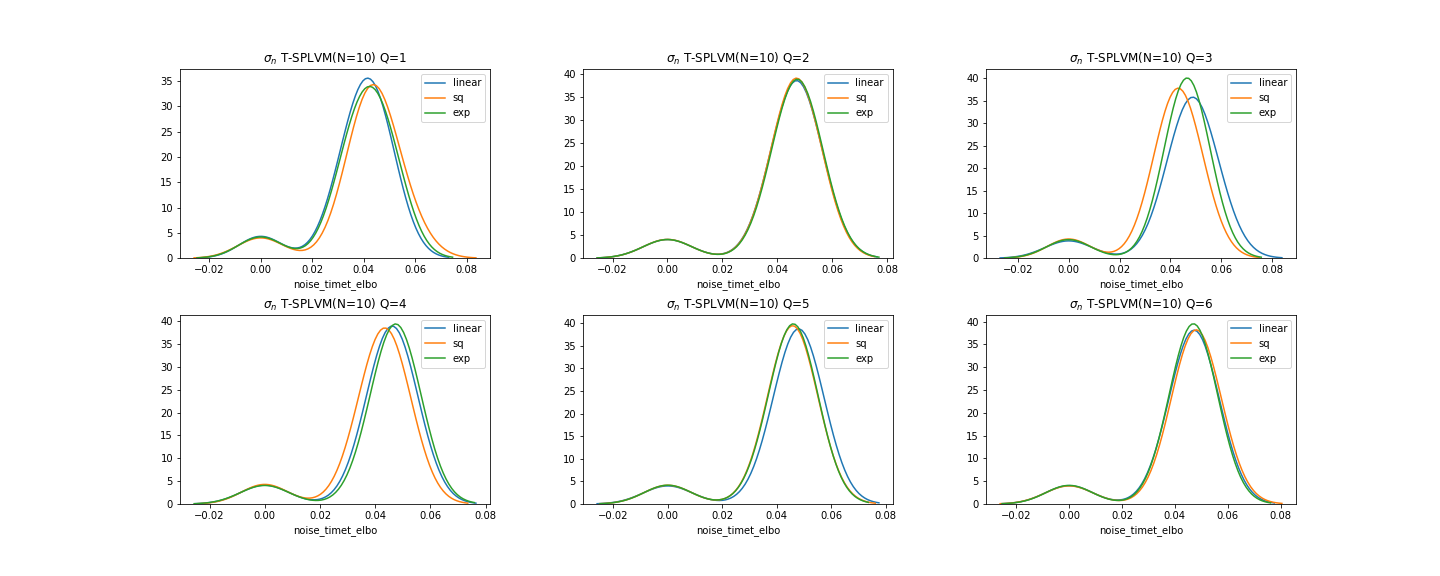
\includegraphics[width=7in]{img/07_4/noise_timet_elbo.png}
	\caption[]{}
	\label{fig:tsplvm_noise}
\end{figure}
Figure \ref{fig:tsplvm_variance} follows, displaying the same unhealthy behavior as the data space process variance did in the T-GPLVM chapter \ref{res:time}. The entries of the covariance matrix then also show unexpected kernel density estimates, ranging to extremely high values. This leads to the conclusion, that the T-SPLVM model still lacks in quality. 
\begin{figure}
	\centering
	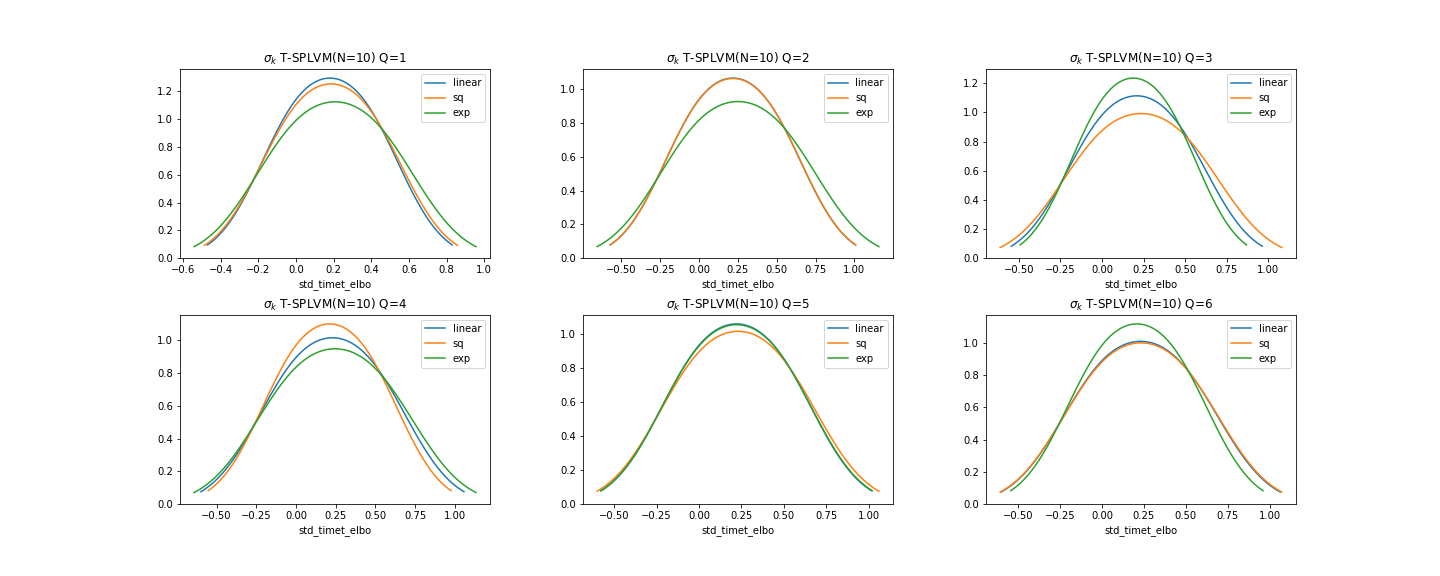
\includegraphics[width=7in]{img/07_4/std_timet_elbo.png}
	\caption[]{}
	\label{fig:tsplvm_variance}
\end{figure}
\begin{figure}
	\centering
	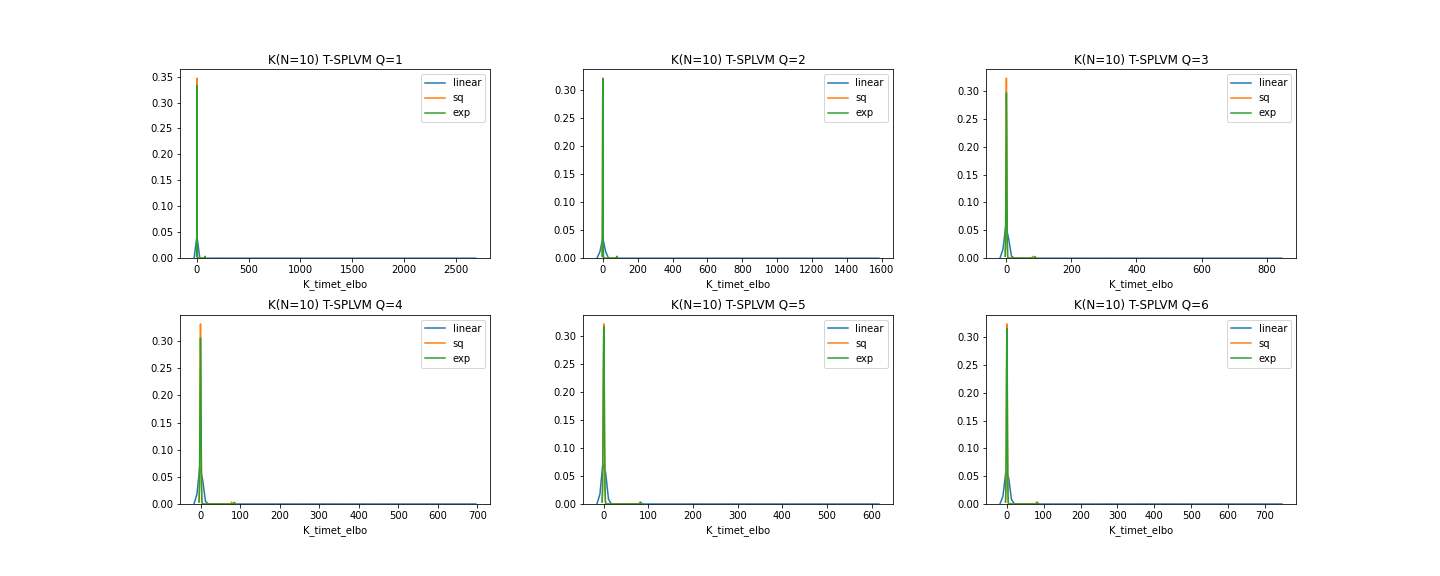
\includegraphics[width=7in]{img/07_4/K_timet_elbo.png}
	\caption[]{}
	\label{}
\end{figure}
Checking the ELBO and $R^2$ values, after identifying erroneous behavior is but a formality, still it is easy to see that the model, scoring comparably to the T-GPLVM model, is not able to compete with the GPLVM or SPLVM model. Here, as the initial expectation suggests, the linear kernel performs considerably worse than the more sophisticated kernels. 
\begin{figure}
	\centering
	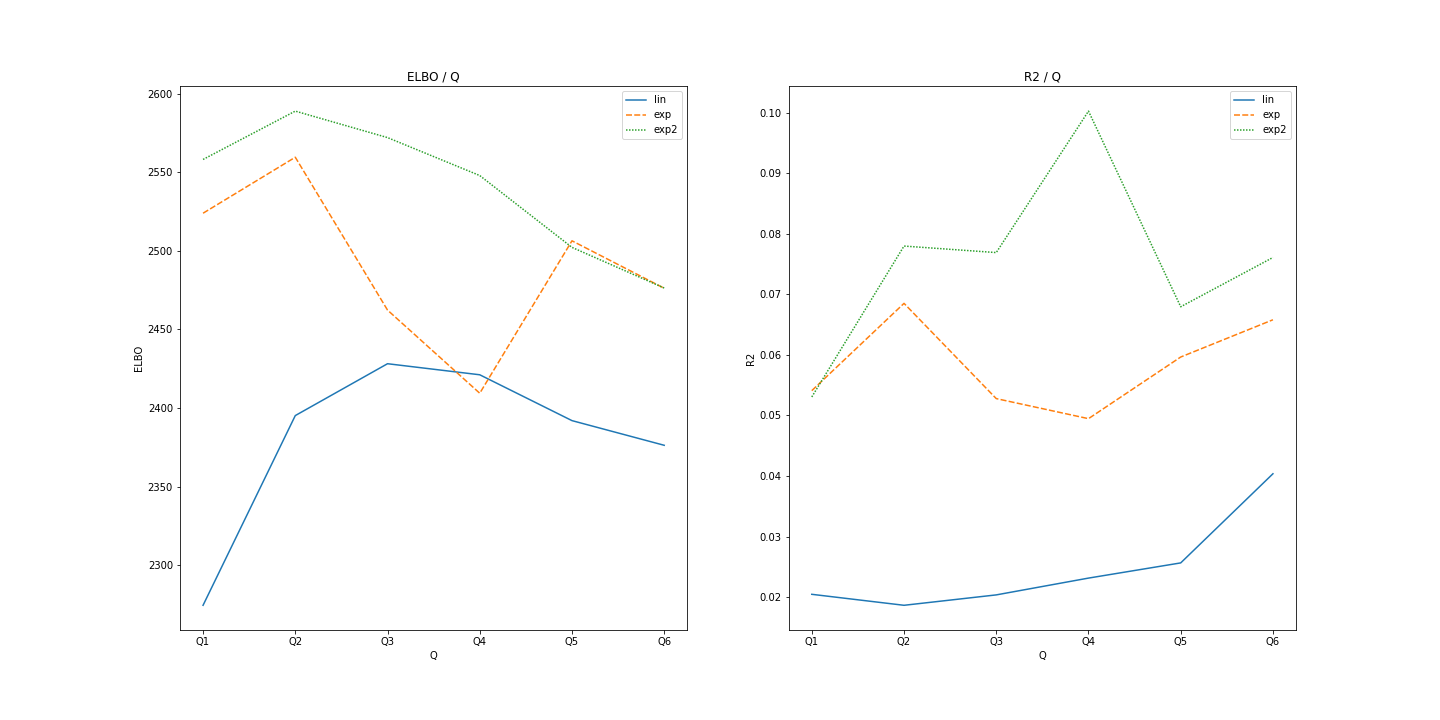
\includegraphics[width=7in]{img/07_4/modelTIMET_Qs.png}
	\caption[]{}
	\label{fig:tsplvm_ELBO_R2}
\end{figure}
The second to last test of the model, looking at slope and intercept distributions, again proves this model as not competitive. While intercepts, as with all models, are close enough to the desired value of 0 to meet expectations.
\begin{figure}
	\centering
	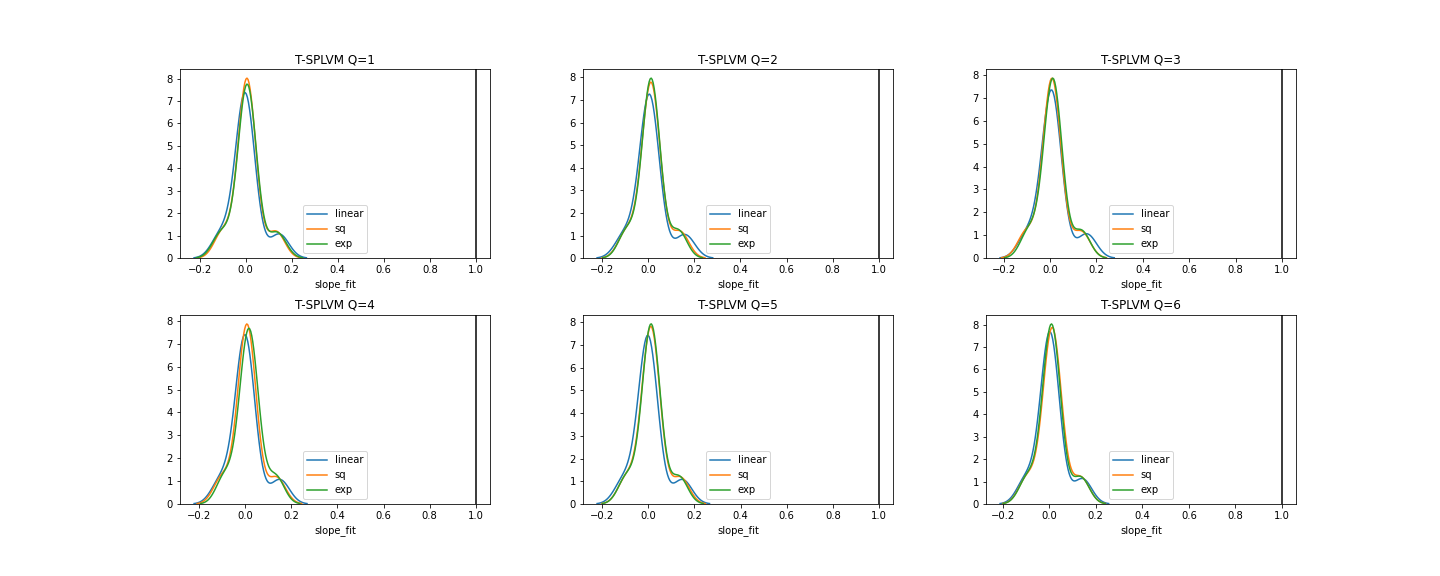
\includegraphics[width=7in]{img/07_4/slope_fit_timet_elbo.png}
	\caption[]{}
	\label{fig:tsplvm_slopes}
\end{figure}
\begin{figure}
	\centering
	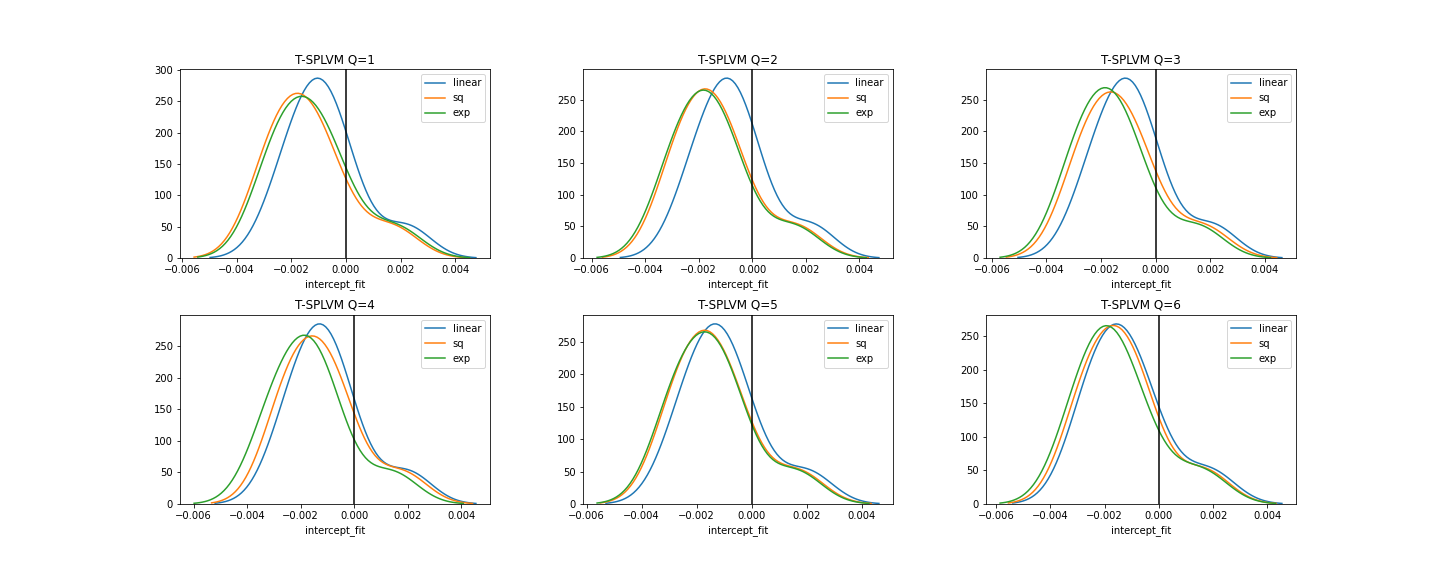
\includegraphics[width=7in]{img/07_4/intercept_fit_timet_elbo.png}
	\caption[]{}
	\label{fig:tsplvm_intercepts}
\end{figure}
The last test of the model, comparing Y-$\hat{Y}$-pair plots \ref{fig:tsplvm_pairs} provides us with the evidence to also not consider this model for further evaluation, showing no behavior close to the expectation. 
\begin{figure}%fig:gplvm_N120_pairs
	\centering
	\begin{subfigure}[l]{0.3\textwidth}
		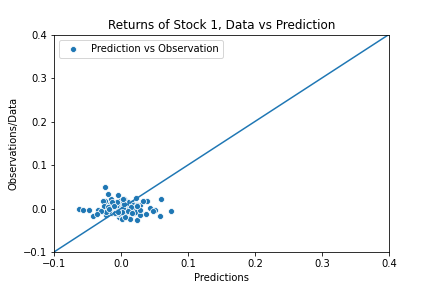
\includegraphics[width=\textwidth]{img/07_4/timet_elbo/Q1_kernel1_stock1_scatter.png}
	\end{subfigure}
	\begin{subfigure}[c]{0.3\textwidth}
		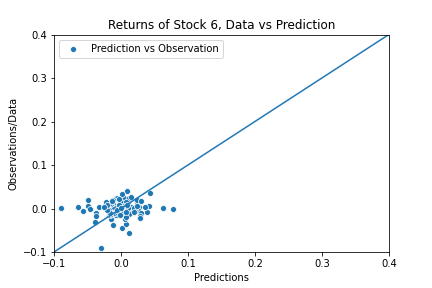
\includegraphics[width=\textwidth]{img/07_4/timet_elbo/Q1_kernel1_stock6_scatter.png}
	\end{subfigure}
	\begin{subfigure}[r]{0.3\textwidth}
		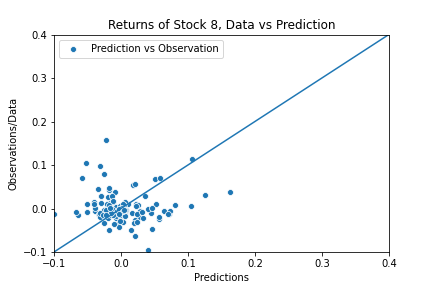
\includegraphics[width=\textwidth]{img/07_4/timet_elbo/Q4_kernel2_stock8_scatter.png}
	\end{subfigure}
	\caption[Y-$\hat{Y}$ pair plots for N=10 with the T-SPLVM model]{Plots from the SPLVM reconstruction with the $N=10$, $D=250$ dataset.}
	\label{fig:tsplvm_pairs}
\end{figure} 
We find defective behavior to hold for all examples of these plots, in all variants of the model. 